\subsection{Filterstufe}\label{sec:filterstufe}
Nachdem die Steuerungseinheit gezeigt wurde, kann nun die Ausgangsstufe erläutert werden. Bevor das Signal verstärkt wird, durchläuft es eine Filterstufe, bestehend aus einer Spule $L$ und einem Kondensator $C$. Das Filter hat die Aufgabe das PWM-Signal des Mikrocontrollers zu filtern und den DC-Anteil zu entfernen. Zusätzlich wird der Mikrocontroller noch vom System entkoppelt. Das wird mit $100\mu F$-Elektrolytkondensatoren an jedem PWM-Ausgang erzielt. Sie werden jeweils seriell geschaltet. Die Dimensionierung der Komponenten wurde mit der nachfolgenden Grundgleichung \ref{eq:LC Filter} durchgeführt:

\begin{equation}
f_g = \frac{1}{2\cdot \pi \cdot \sqrt{L\cdot C}}
\label{eq:LC Filter}
\end{equation}

Nun wird die Grenzfrequenz $f_g$ mit $20 kHz$ festgelegt und ein Kondensator $C$ mit dem Wert $1\mu F$ gewählt. Jetzt kann die Gleichung \ref{eq:LC Filter} nach der Spule $L$ umgestellt werden:

\begin{equation}
L = \frac{1}{(2\cdot \pi \cdot f_g)^2\cdot C }
\label{eq:LC Filter nach L}
\end{equation}

Durch das Einsetzen der Werte für $C$ und $f_g$ in Gleichung \ref{eq:LC Filter nach L} erhält man die folgende Induktivität für die Spule:

\begin{equation}
L = \frac{1}{(2\cdot \pi \cdot f_g)^2\cdot C } = \frac{1}{(2\cdot \pi \cdot 20 kHz)^2\cdot 1 \mu F } = 63.33\mu H
\label{eq:LC Filter nach L 1}
\end{equation}

Unter Einhaltung der {\glqq E12-Reihe\grqq} wird nun der berechnete Wert von $63.33\mu H$ auf den nächstliegenden Wert der Reihe von $68\mu H$ gesetzt. Da es nun zu Abweichungen in der Berechnung kommt, muss die Grenzfrequenz $f_g$ noch mit den bestimmten Bauteilwerten von $L$ und $C$ zurückgerechnet werden. Durch das Einsetzen der Werte in die Gleichung \ref{eq:LC Filter}, erhält man die nachfolgende Grenzfrequenz $f_g$:

\begin{equation}
f_g = \frac{1}{2\cdot \pi \cdot \sqrt{L\cdot C}} = \frac{1}{2\cdot \pi \cdot \sqrt{68\mu H \cdot 1 \mu F}} = 19.3 kHz
\label{eq:LC Filter 1}
\end{equation}

Es ist eine Differenz zur ursprünglichen Annahme von $700 Hz$ zu erkennen, die jedoch in dieser Anwendung vernachlässigt werden kann. In Abbildung \ref{fig:Filterstufe} ist der Aufbau zu sehen. Dabei ist $C_{1}$ der Entkopplungskondensator und $L_{1}$ und $C_{2}$ bilden zusammen die Filterstufe. Rechts ist der Ausgang zur Verstärkerstufe zu sehen, welche im nächsten Kapitel beschrieben wird.


\begin{figure}[H]
	\begin{center}
		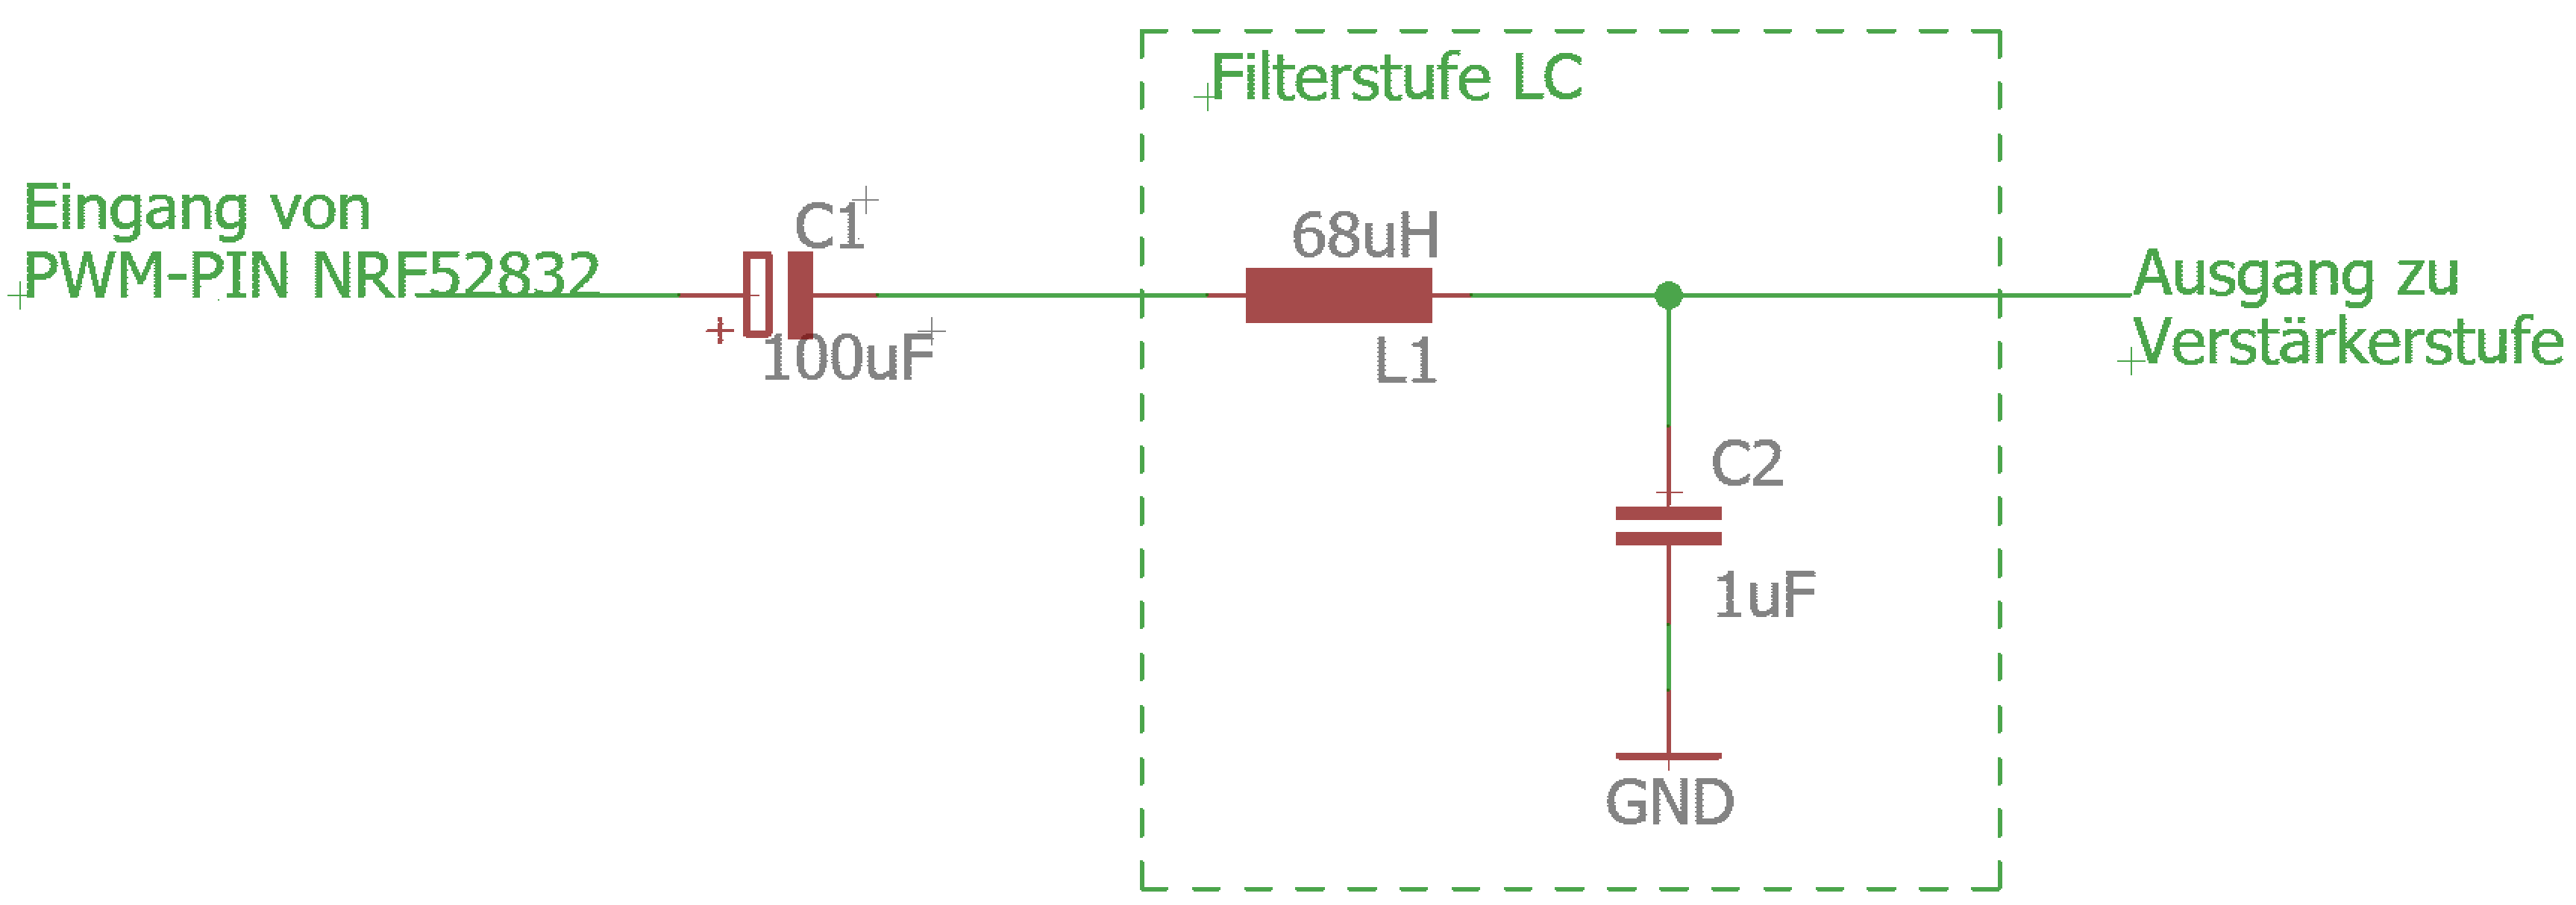
\includegraphics[width=\textwidth]{data/Schema_Filterstufe.png}
		\caption[Schema der LC-Filterstufe]{Schema der LC-Filterstufe}
		\label{fig:Filterstufe}
	\end{center}
\end{figure}

\subsection{Verstärkerstufe} \label{sec:verstaerkerstufe}
Mit einer Verstärkerstufe lassen sich auf einfache Art und Weise Signale jeglicher Form verstärken. Sie eignen sich bestens, um den Ausgang eines Mikrocontrollers entsprechend aufzubereiten, da die Ausgangsseite meist sehr niedrige Ströme aufweist. Dadurch kann dem Knochenschallaktor genügend Energie zur Verfügung gestellt werden. Prinzipiell gibt es zwei Arten von Verstärkern. Entweder erfolgt die Umsetzung digital oder analog. Beide erfüllen die gleiche Aufgabe, weisen jedoch bezüglich Wirkungsgrad einen deutlichen Unterschied auf. Die digitale Variante weist ungefähr einen Wirkungsgrad von 90$\%$ auf \cite{BoneConductorAdafruit}, während die analoge Variante einen maximalen Wirkungsgrad im Bereich der Leistungsanpassung erzielt \cite{Niklaus_Skript}. Aus diesem Grund wird ein digitaler Verstärker (Class-D-Verstärker) in der Anwendung implementiert. Die Wahl fiel auf den Stereo-Amplifier MAX 98306. Der Verstärker hat in Betrieb einen Stromverbrauch von $143mA$ und eine Speisespannung von $3.3V$. Somit hat er einen Leistungsverbrauch von $471.9 mW$. Im Standby benötigt er lediglich $2 mA$ und somit $6.6 mW$\cite{Verstaerker}. In Abbildung \ref{fig:verstaerkerstufe} ist der schematische Aufbau des Verstärkers dargestellt.

\begin{figure}[H]
	\begin{center}
		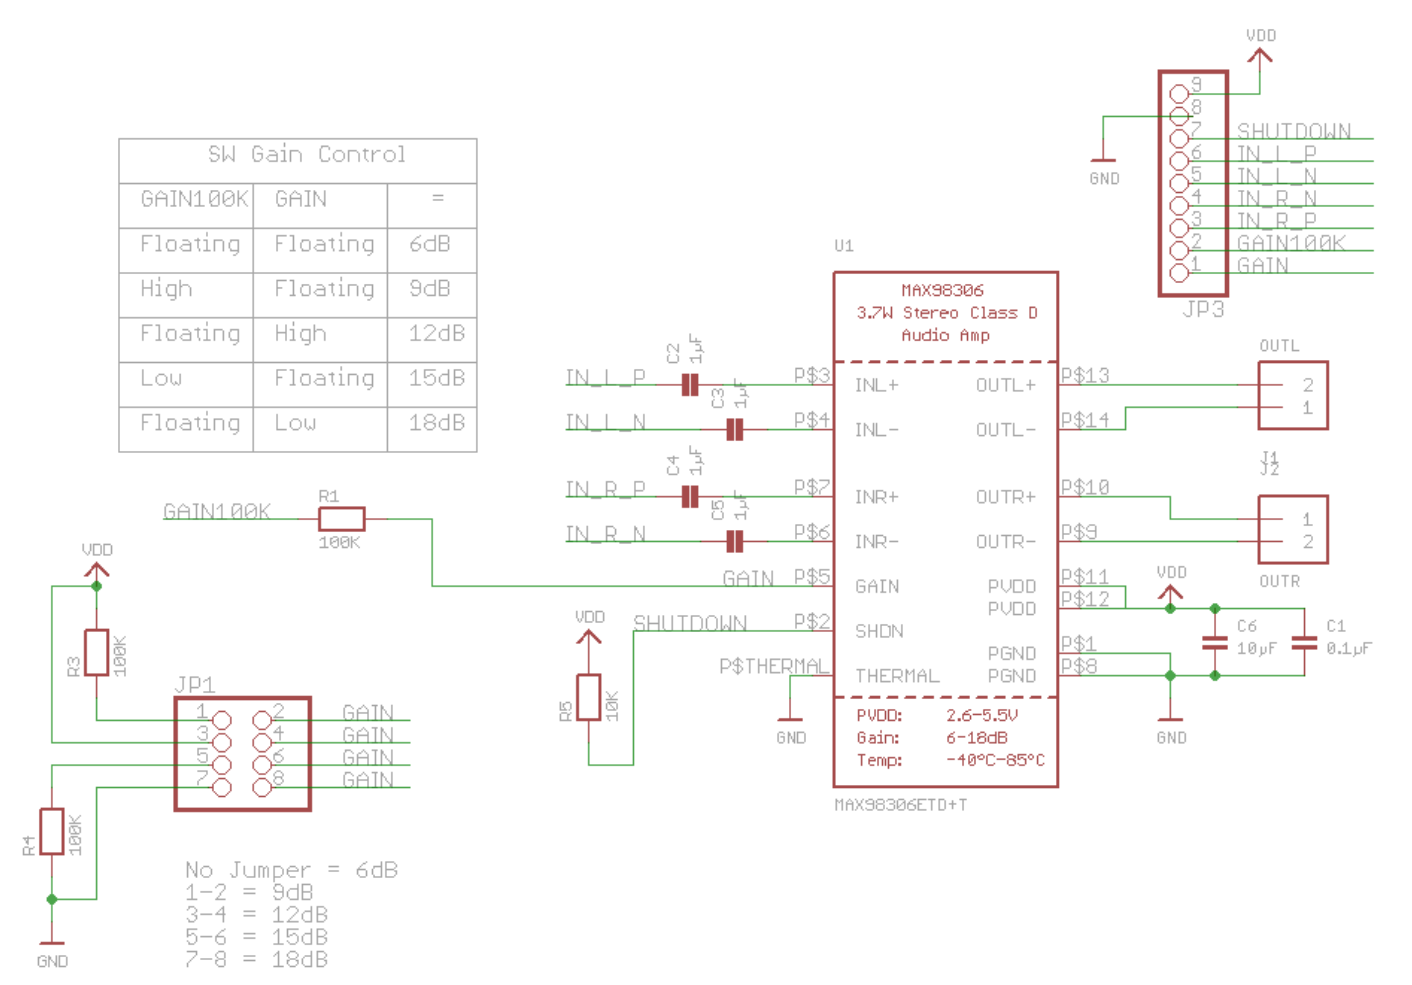
\includegraphics[width=\textwidth]{data/Schema_Verstaerkerstufe.png}
		\caption[Verstärkerstufe \cite{Verstaerker_Schema}]{Schema der Verstärkerstufe} %picture caption
		\label{fig:verstaerkerstufe}
	\end{center}
\end{figure}

\subsection{Knochenschallaktor} \label{sec:knochenschallaktor}
Nachdem das vom Mikrocontroller ausgegebene Audio-File über die Filter- und Verstärkerstufe entsprechend aufbereitet wurde, kann nun die Audiodatei über einen sogenannten Knochenschallaktor ausgegeben werden. Der Aktor arbeitet nach dem Prinzip der Weiterleitung von Schall-Schwingungen oder auch Vibrationen. Dadurch lässt sich der ursprüngliche Gehörgang umgehen und die Schwingungen werden über den Schädelknochen an das Innenohr übertragen. Dies verbessert auch die Hygiene der Anwendung, da kein direkter Kontakt mit dem Gehörgang stattfindet\cite{Knochenschall}. Falls weitere Informationen zur Knochenschalltechnologie gewünscht werden, wird an dieser Stelle auf die Quelle \cite{Knochenschall_HDM_Stuttgart} verwiesen. Für die Anwendung im Dōjō wird ein Knochenschallaktor des Herstellers Adafruit verwendet, welcher in der Abbildung \ref{fig:knochenschallAda} ersichtlich ist.

\begin{figure}[H]
	\begin{center}
		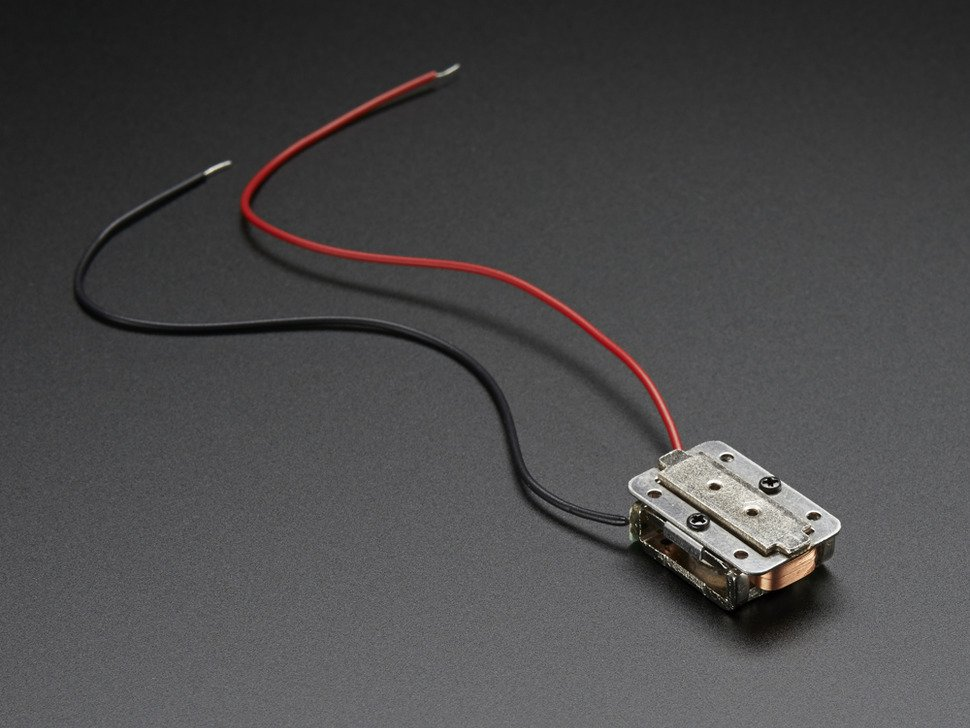
\includegraphics[width=0.6\textwidth]{data/KnochenschallaktorAdafruit1.jpg}
		\caption[Knochenschallaktor \cite{BoneConductorAdafruit}]{Knochenschallaktor von Adafruit} %picture caption
		\label{fig:knochenschallAda}
	\end{center}
\end{figure}

Das ausgewählte Bauteil eignet sich bestens für die Verwendung im Dōjō. Mit einem Gewicht von $9.6 g$ und den Dimensionen $(14x21,5x7,9) mm$ lässt sich der Aktor gut in das bestehende Gehäuse implementieren \cite{BoneConductorAdafruit}. Weiter ist das Bauteil relativ kostengünstig im Handel erhältlich und kann $1W_{RMS}$ Leistung liefern, was sich dann in der Lautstärke bemerkbar macht. Nach ausführlichen Recherchearbeiten konnten keine wirklichen Alternativen ausgemacht werden. Meist befindet sich die Technologie noch in der Entwicklungsphase oder fällt aufgrund des Preises aus der Auswahlmöglichkeit.
